\documentclass[12pt]{report}
\usepackage{scribe,graphicx,graphics}
\newcommand{\prox}[2]{\text{prox}_{#1}\left(#2\right)} 
\newcommand{\lone}[1]{\left\Vert #1\right\Vert_1} 
\newcommand{\ltwo}[1]{\left\Vert #1\right\Vert_2} 
\newcommand{\lzero}[1]{\left\Vert #1\right\Vert_0} 
\newcommand{\sign}[1]{\text{sign}\left(#1\right)}

\newcommand{\expct}[1]{\mathbb{E}\left(#1\right)}
\newcommand{\expctd}[2]{\mathbb{E}_{#1}\left(#2\right)}
\newcommand{\abs}[1]{\left\vert#1\right\vert}
\newcommand{\defeq}{\mathrel{\mathop:}=}
\newcommand{\eqdef}{=\mathrel{\mathop:}}
\newcommand{\rank}[1]{\text{rank}\left( #1 \right)}
\newcommand{\norm}[2]{{\left\Vert #1 \right\Vert}_{#2}}
\newcommand{\eig}[1]{\text{eig}\left( #1 \right)}
\newcommand{\prob}[1]{p\left( #1 \right)}
\newcommand{\bigprob}[1]{\mathbb{P}\left( #1 \right)}
\newcommand{\bigprobd}[2]{\mathbb{P}_{#1}\left( #2 \right)}
\newcommand{\probd}[2]{p_{{#1}}\left( #2 \right)}
\newcommand{\cprob}[2]{p\left( #1 \vert #2 \right)}
\newcommand{\cprobd}[3]{p_{#1\vert #3}\left( #2 \vert #3 \right)}
\newcommand{\set}[1]{\left\lbrace #1 \right\rbrace}
\newcommand{\rv}[2]{p_{#1}\left( #2 \right)}
\newcommand{\crv}[2]{f_{#1}\left( #2 \right)}
\newcommand{\cdf}[2]{F_{#1}\left( #2 \right)}
\newcommand{\epct}[1]{\mathbb{E}\left( #1 \right)}
\newcommand{\var}[1]{\text{var}\left( #1 \right)}
\newcommand{\vard}[2]{\text{var}_{#1}\left( #2 \right)}
\newcommand{\cvar}[2]{\text{covar}\left( #1, #2 \right)}
\newcommand{\epctd}[2]{\mathbb{E}_{#1}\left(#2\right)}

\newcommand{\bdy}{\mathbf{y}}
\newcommand{\bdz}{\mathbf{z}}
\newcommand{\bdx}{\mathbf{x}}
\newcommand{\bdu}{\mathbf{u}}
\newcommand{\bdH}{\mathbf{H}}
\newcommand{\bdr}{\mathbf{r}}
\newcommand{\lrr}{\substack{\geq\\ \leq}}
\usepackage{float}
\usepackage{bm}
\usepackage{bbm}
\usepackage{tikz}
\usepackage{mathtools}
\usepackage{bbm}
\usepackage{epstopdf}
\usepackage[mathscr]{euscript}
\usepackage{mathrsfs}
\usepackage{enumerate}
\usepackage[numbers,super,sort&compress]{natbib}
\usepackage{bibentry}
\usepackage{setspace}
\PassOptionsToPackage{hyphens}{url}\usepackage{hyperref}
\course{MIT 6.437} 	
\coursetitle{Inference and Information}	
\semester{Spring 2018}
\lecturer{} % Due Date: {\bf Mon, Oct 3 2016}}
\lecturetitle{Project}
\lecturenumber{1}   
\lecturedate{}    

\usepackage{algorithm}% http://ctan.org/pkg/algorithms
\usepackage{algpseudocode}% http://ctan.org/pkg/algorithmicx
\newcommand\numberthis{\addtocounter{equation}{1}\tag{\theequation}}
\makeatletter
\def\BState{\State\hskip-\ALG@thistlm}
\makeatother
% Insert your name here!
\scribe{Student Name: Jon Paul Janet}

\begin{document}


\maketitle

\paragraph{Problem 1}
$ $ \\
\begin{enumerate}[a]
	\item Since $f$ is one-to-one:
	\begin{align*}
	y_i &= f(x_i)\quad \forall i \in \left\lbrace 1, 2,\hdots, n \right\rbrace\\
	\probd{\bdx}{\bdx = \left\lbrace x_1, x_2, \hdots x_n \right\rbrace} &= P(x_1, x_2, \hdots, x_n) \\
	&= P(x=x_1) P(x_2, \hdots, x_n \vert x_1 =x_1 )\\
	&=\probd{x}{x_1}\cprobd{x_2}{x_2}{x_3}\cprobd{x_3}{x_3}{x_4}\hdots \cprobd{x_n}{x_n}{x_{n-1}}\\
	&= \probd{x}{x_1} M_{(x_2),(x_3)}M_{(x_3),(x_4)}\hdots M_{(x_{n-1}),(x_n)}\\
	\end{align*}
	Where $M_{(x_i),(x_j)}$ represents the transition probability from the symbol of $x_i$ to the symbol of $x_j$. The probability of $y$ can then be expressed, knowing $f$:
	\begin{align*}
	\cprobd{{y_1}}{y_1}{f}&=\sum_{ \substack{x': f(x') = y_1 \\ x' \in \mathcal{A} }} p_{x}(x')= \probd{x}{f^{-1}(y_1)}\\
	\cprobd{\bdy}{\bdy}{f}&= \probd{\bdx}{f^{-1}(\bdy)}\\
	&= \probd{x}{f^{-1}(\bdy)_1} M_{(f^{-1}(\bdy)_2),(f^{-1}(\bdy)_3)}M_{(f^{-1}(\bdy)_3),(f^{-1}(\bdy)_4)}\hdots M_{(f^{-1}(\bdy)_{n-1}),(f^{-1}(\bdy)_n)}\\
	\end{align*}
\hrule
\item 
	\begin{align*}
	\cprobd{f}{f}{\bdy}&=\frac{	\cprobd{\bdy}{\bdy}{f} \probd{f}{f}}{\probd{\bdy}{\bdy}}\\
	\probd{\bdy}{\bdy} &= \sum_{\bdy}	\cprobd{\bdy}{\bdy}{f} \probd{f}{f}
	\end{align*}
	As it will be useful later:
	\begin{align*}
\cprobd{f}{f}{\bdy}&=\frac{	\cprobd{\bdy}{\bdy}{f} \probd{f}{f}}{\probd{\bdy}{\bdy}}\\
	\implies  \log \cprobd{f}{f}{\bdy} &= \log\cprobd{\bdy}{\bdy}{f} + \log \probd{f}{f}  - \log \probd{\bdy}{\bdy}\\
	&=  \left[\log\probd{x}{f^{-1}(\bdy)_1} + \sum_{i=1}^{n} M_{(f^{-1}(\bdy)_{i-1}),(f^{-1}(\bdy)_{i})}\right] + \log \left\vert \mathcal{A}\right\vert - \log \probd{\bdy}{\bdy}
	\end{align*}
	Here, we can compute $\cprobd{\bdy}{\bdy}{f}$ for any $f$ in terms of the given $M$ and we assume a uniform prior on $f$ across the space of all $28$-key permutations $\mathcal{F}$, i.e. $\probd{f}{f}=\frac{1}{28!}$.
	The map can be defined as 
	\begin{align*}
		\hat{f}_{MAP}(\bdy) &= \arg\max_{f\in\mathcal{F}}\left[\cprobd{f}{f}{\bdy}\right]\\
		&=\arg\max_{f\in\mathcal{F}}\left[\frac{	\cprobd{\bdy}{\bdy}{f} \probd{f}{f}}{\probd{\bdy}{\bdy}}\right]\\
		&= \arg\max_{f\in\mathcal{F}}\left[\cprobd{\bdy}{\bdy}{f}\probd{f}{f}\right] =\arg\max_{f\in\mathcal{F}}\left[\log\cprobd{\bdy}{\bdy}{f}\probd{f}{f}\right]\\
    \end{align*}
    \hrule
  
    \item The  above minimization is overt the set $\mathcal{F}$ which is discrete and very large (the 28-permutohedron), with $\left\vert\mathcal{F} \right\vert =28!$, meaning the the optimization is NP-hard and unfeasibly-high dimensional
    \hrule
	\end{enumerate}
\newpage
\paragraph{Problem 2}
$ $ \\
\begin{enumerate}[a]
	\item let $f^{(1)}$, $f^{(2)}$ correspond to two randomly drawn permuations from $\mathcal{F}$
	\begin{align*}
	\bigprob{f^{(1)}_{i}\neq f^{(2)}_i,\:f^{(1)}_{j}\neq f^{(2)}_j,  \: f_k = f_k\: \forall k \neq i,j }
	\end{align*}
	Clearly there are ${{N}\choose{2}}$ pairs of $i,j$ that can be interchanged starting from $f^{1}$, and $N!-1$ other permutations to select $f^{(2)}$ from. Therefore for two uniformly selected $f^{(1)},f^{(2)}\in \mathcal{F}$: 
	\begin{align*}
	\bigprob{f^{(1)}_{i}\neq f^{(2)}_i,\:f^{(1)}_{j}\neq f^{(2)}_j,  \: f_k = f_k\: \forall k \neq i,j } &= \frac{{{N}\choose{2}}}{N!-1} 
	\end{align*}
	Let the set of $1-$pair exchanged sequences from a given $f\in\mathcal{F}$ be denoted $\mathcal{F}_1(f)$, with $\left\vert \mathcal{F}_1(f)\right\vert={{N}\choose{2}}<<\left\vert \mathcal{F}\right\vert=N!$. This also us to define a uniform proposal density $V(f'\vert f)$:
	\begin{align*}
		{V}_{f'\vert f}(f'\vert f) = \begin{cases}
		{{N}\choose{2}}^{-1} & f'\in \mathcal{F}_{1}(f) \\
		0 & \text{otherwise}
		\end{cases}
	\end{align*}
	Note that this transition probability is symmetric, i.e. ${V}_{f\vert f}(f^{(k+1)}\vert f^{(k)})=V_{f\vert f}(f^{(k)}\vert f^{(k+1)})$ an so the detailed balance equations will be satisfied for this choice.
	\hrule
	\item The MHMC algorithm is as follows:
	\begin{enumerate}[1]
		\item Generate $f^{(0)}$ from $\mathcal{F}$ according to $\probd{f}{f}$ (uniform)
		\item for $k=0,1,\hdots,n$:
		\begin{enumerate}[i]
			\item generate $f'$ from $\mathcal{F}_1$ according to $V(f'\vert f^{(k)})$ (uniform on $\mathcal{F}_{1}(f^{(k)}$)
			\item calculate $\alpha = \min \left[1,\frac{\cprobd{f}{f'}{\bdy}{V}(f^{(k)}\vert f')}{\cprobd{f}{f^{(k)}}{\bdy}{V}(f'\vert f^{(k)})}\right]=\min \left[1,\frac{\cprobd{f}{f'}{\bdy}}{\cprobd{f}{f^{(k)}}{\bdy}}\right]$. 
			\item generate $a$ from a Bernouli distribution with parameter $\alpha$, $a\sim\mathcal{B}(\alpha)$. 
			\item If $a = 1$, $f^{(k+1)}=f'$, else $f^{(k+1)}=f^{(k)}$
			\item repeat until $k=n$
		\end{enumerate}
	\hrule
	\item 
	\begin{algorithm}
		\caption{My algorithm}\label{euclid}
		\begin{algorithmic}[1]
			\Procedure{MyProcedure}{}
			\State $\textit{stringlen} \gets \text{length of }\textit{string}$
			\State $i \gets \textit{patlen}$
			\BState \emph{top}:
			\If {$i > \textit{stringlen}$} \Return false
			\EndIf
			\State $j \gets \textit{patlen}$
			\BState \emph{loop}:
			\If {$\textit{string}(i) = \textit{path}(j)$}
			\State $j \gets j-1$.
			\State $i \gets i-1$.
			\State \textbf{goto} \emph{loop}.
			\State \textbf{close};
			\EndIf
			\State $i \gets i+\max(\textit{delta}_1(\textit{string}(i)),\textit{delta}_2(j))$.
			\State \textbf{goto} \emph{top}.
			\EndProcedure
		\end{algorithmic}
	\end{algorithm}
	\end{enumerate}

	\end{enumerate}

\newpage
\paragraph{Problem 3}
$ $ \\
The inference task was repeated for $50$ random initializations and run for $5000$ iterations each time.
\begin{enumerate}[a)]
	\item $ $
	\begin{figure}[H]
		\centering
		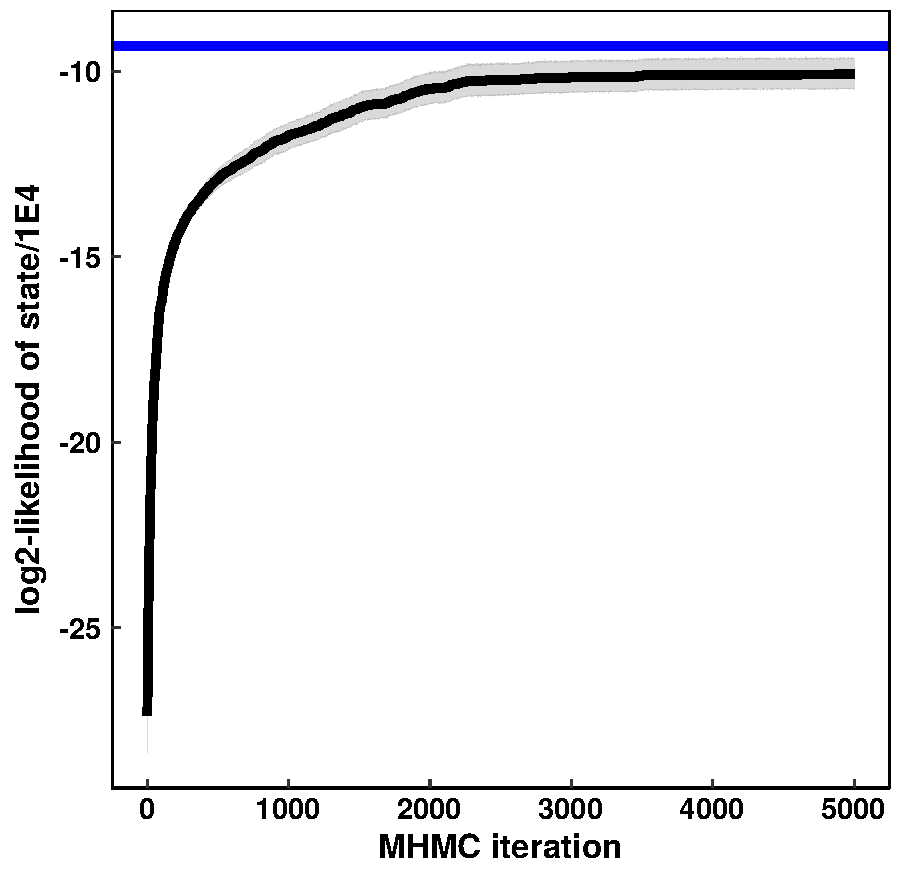
\includegraphics[width=.45\linewidth]{../logl}
		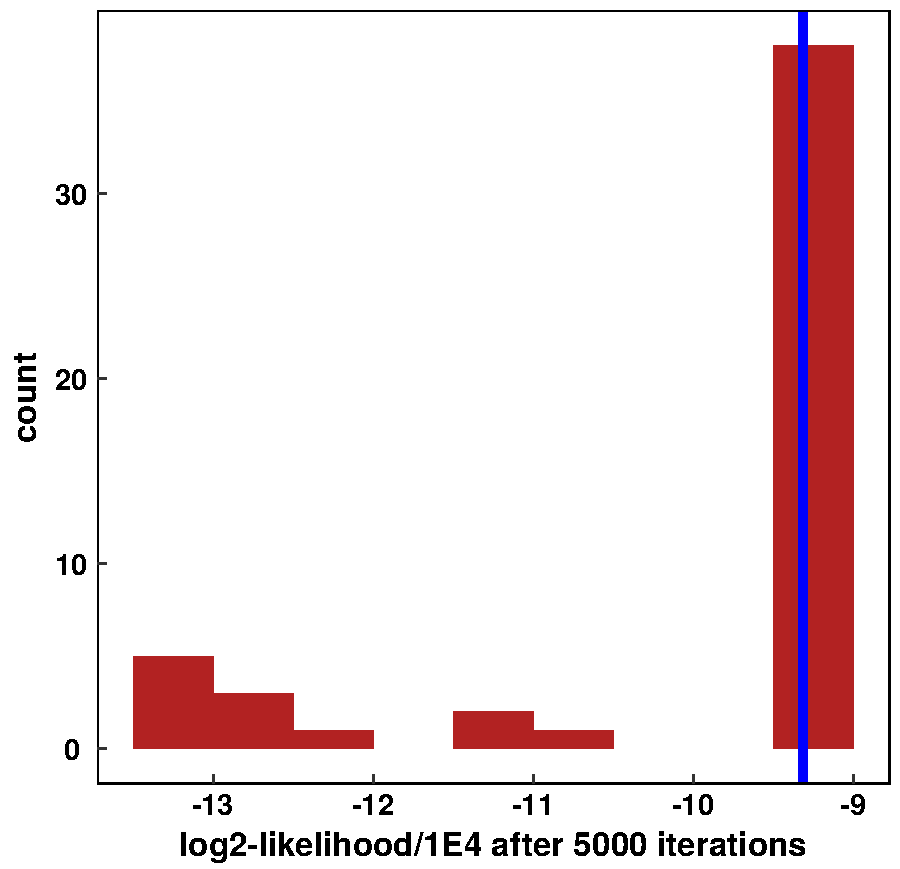
\includegraphics[width=.45\linewidth]{../loglhist} 
		\caption{ (L) Log-likelihood in bits as a function of MHMC iteration, showing average over 50 random initializations and $95\%$ confidence interval based on non-parametric bootstrap with $1000$ draws. The blue line shows the log-likelihood of the true cipher. (R) Histogram of log-likelihood after $5000$ iterations showing that the correct minimum is obtained in $76\%$ of random initializations. \label{Fig:lolg}}
	\end{figure}
	\hrule 
	\item $ $
	\begin{figure}[H]
	\centering
	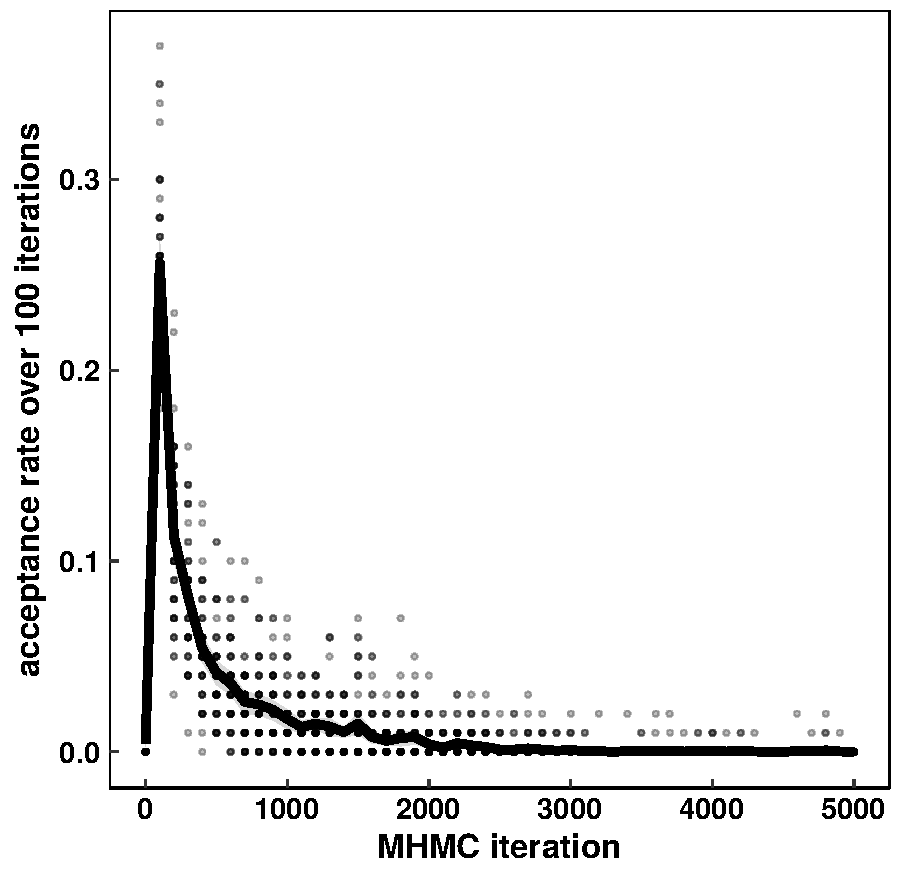
\includegraphics[width=.45\linewidth]{../AR} 
	\caption{Average accept rate over 100 iterations as a function of MHMC iteration, showing average over 50 random initializations and $95\%$ confidence interval based on nonparametric bootstrap. Individual runs shown as dots. \label{Fig:arg}}
	\end{figure}
	\hrule
	\item $ $
	\begin{figure}[H]
	\centering 
	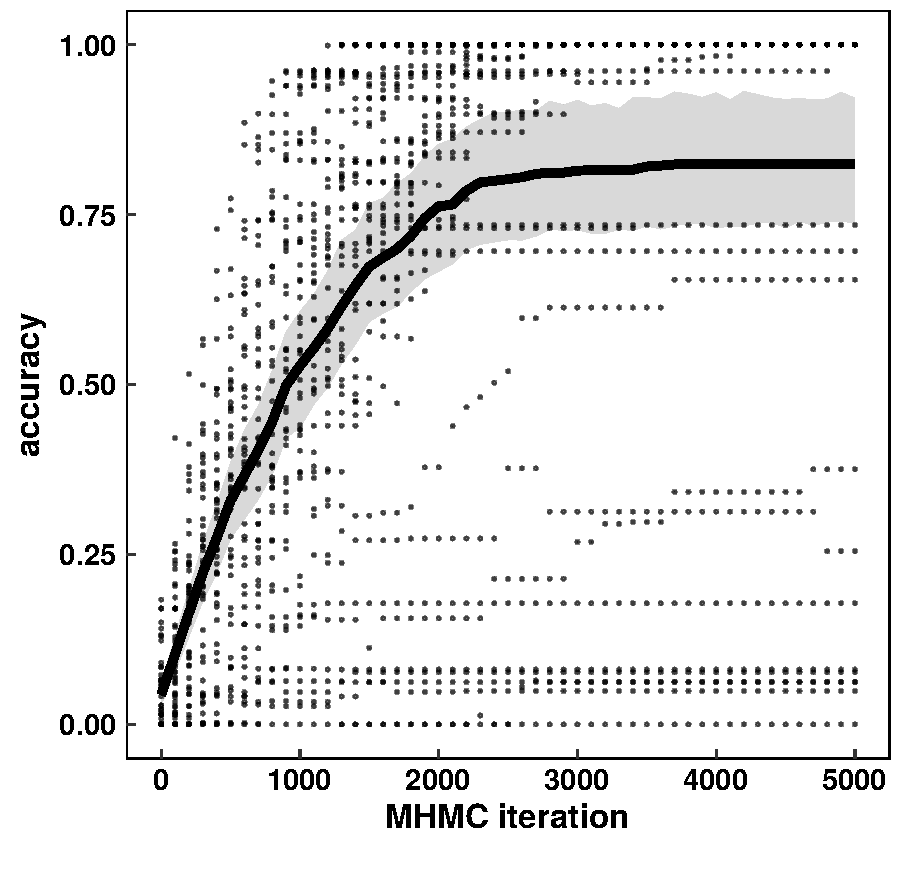
\includegraphics[width=.45\linewidth]{../acc} 
	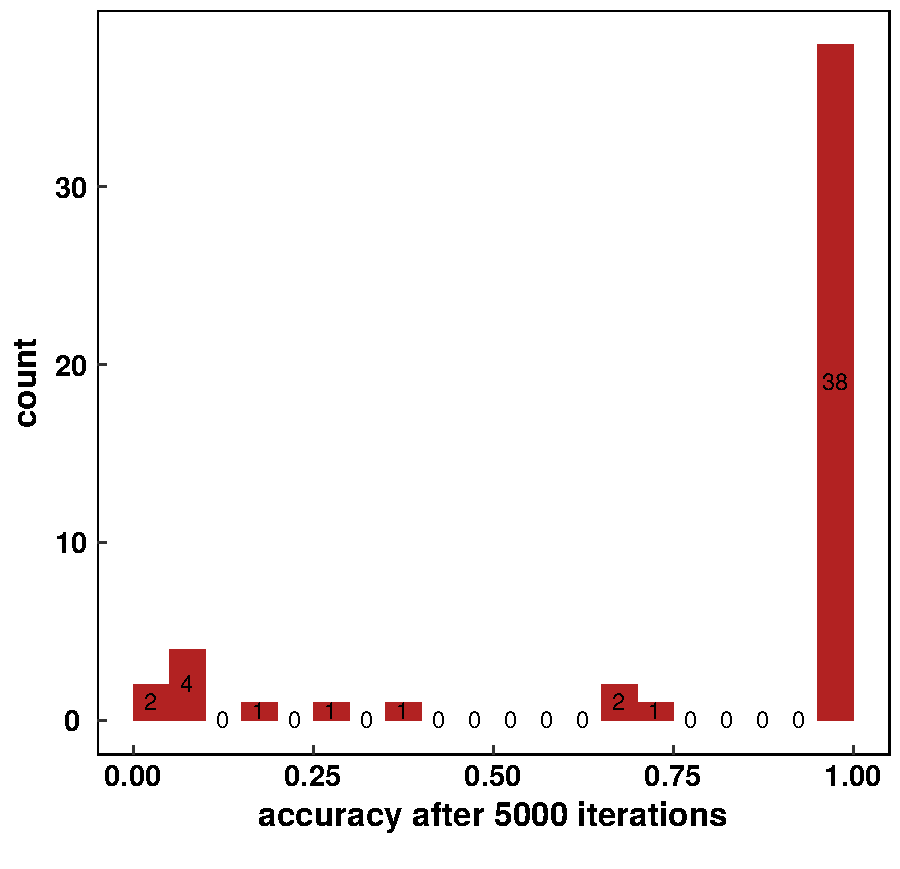
\includegraphics[width=.45\linewidth]{../acchist} 
	\caption{(L) Accuracy in fraction of correctly decoded characters as a function of MHMC iteration, showing average over 50 random initializations and $95\%$ confidence interval based on non-parametric bootstrap with $1000$ draws. Individual runs shown as dots. (R) Final accuracy after $5000$ iterations showing bin counts for 50 random initializations. The correct answer is obtained in $76\%$ of random initializations.  \label{Fig:accg}}
	\end{figure}
	\hrule
	\newpage
	\item The inference task was repeated, varying the length of the input ciphertext from  $500$ to $27320$ characters (full length). These trials were repeated using $10$ random initializations each. Reducing sequence length makes the inference task more difficult, although the random initial conditions and low number of repeats (in particular for $L=8000$) make the trend less obvious, as evidenced by the large confidence interval obtained. This is expected since the  longer the text, the more sharply peaked the log-likelihood will be around ciphers that produce common letter orders. Additionally, the inference is based on aggregate $2$-gram statistics and it is expected local deviations from these averages will be more extreme (i.e. weak law of large numbers).
	\begin{figure}[H]
			\centering
			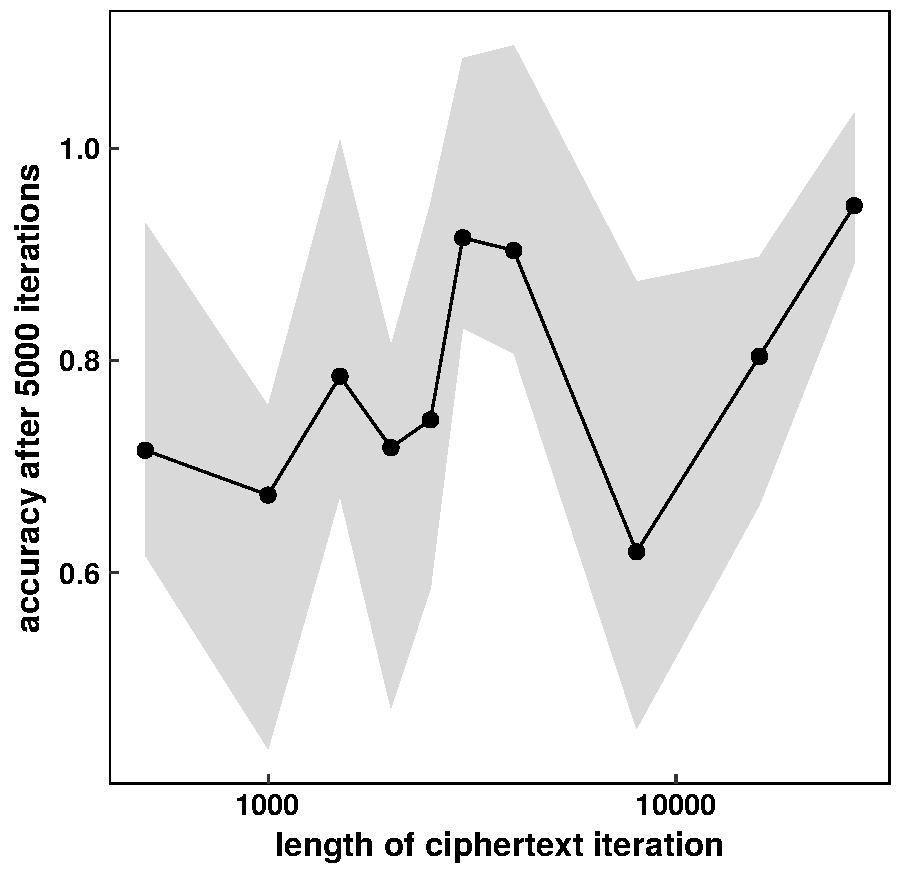
\includegraphics[width=.45\linewidth]{../Lacc}
			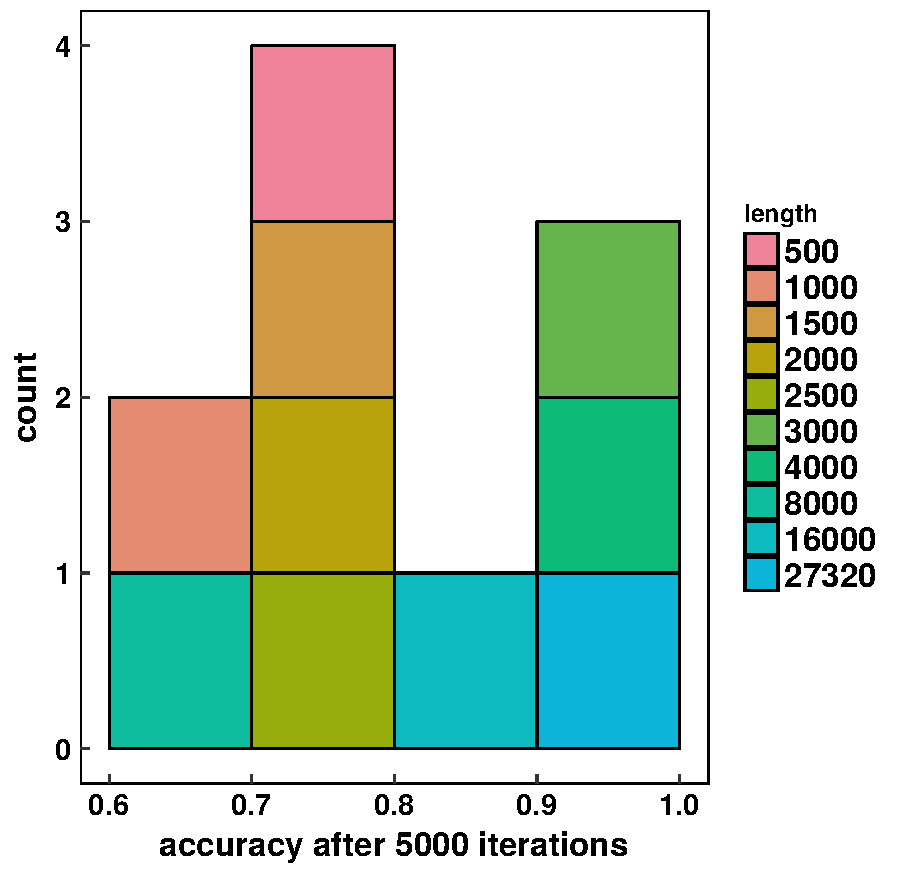
\includegraphics[width=.45\linewidth]{../LaccHist} 
			\caption{ (L) Accuracy in fraction of after 5000 MHMC iterations as a function of ciphertext length, showing average over 10 random initializations and $95\%$ confidence interval based on non-parametric bootstrap with $1000$ draws. (R) Final accuracy after $5000$ iterations grouped by ciphertext length, showing bin counts for 10 random initializations. While the $L=8000$ case is atypical, there is a clear trend towards obtaining high accuracy for longer chains (cool colours concentrate to the right). \label{Fig:Laccg}}
	\end{figure}
	\hrule
	\newpage
	\item The (negative) log-likelihood in bits per character of the decoded plaintext, which is $27320$ characters, increases with iteration and maximizes at a very similar value of $3.41$ compared to the $2$-gram entropy value of $3.32$ suggested by Shannon\cite{shannon1951prediction} for a $27$-symbol alphabet. 
		\begin{figure}[H]
				\centering
				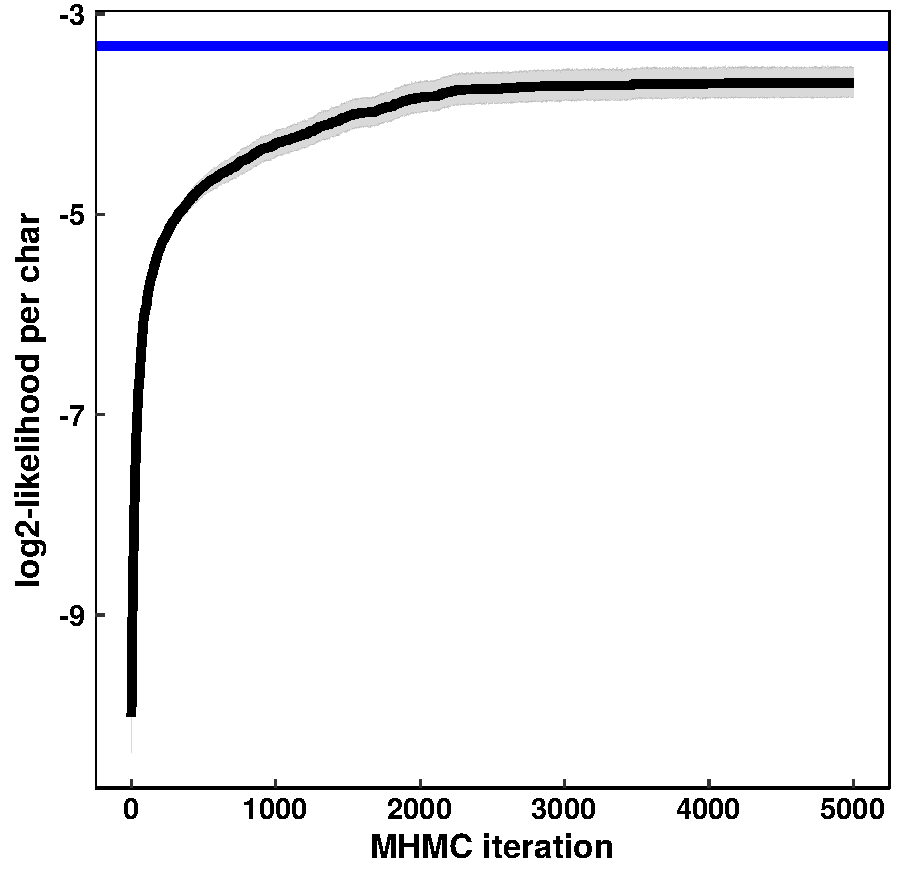
\includegraphics[width=.45\linewidth]{../ent}
				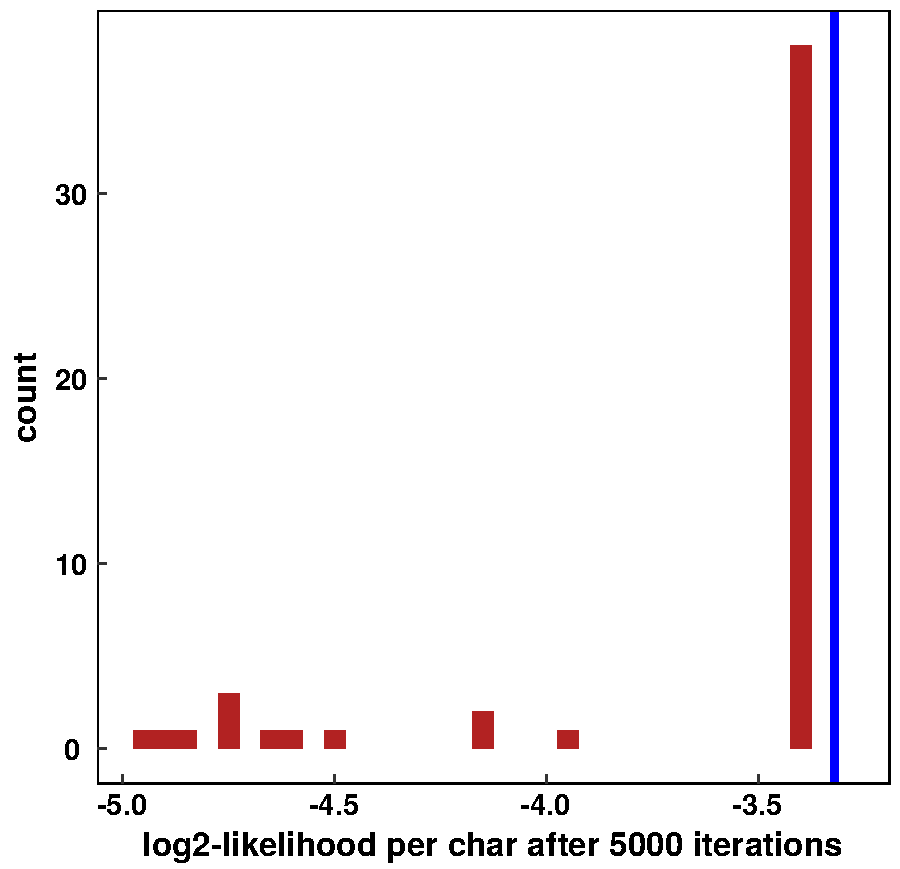
\includegraphics[width=.45\linewidth]{../enthist} 
				\caption{ (L) Log-likelihood in bits per character as a function of MHMC iteration, showing average over 50 random initializations and $95\%$ confidence interval based on non-parametric bootstrap with $1000$ draws. The blue line shows the Shannon $2$-gram entropy\cite{shannon1951prediction}. (R) Histogram of log-likelihood per character after $5000$ iterations showing that most chains converge to to a value near the  Shannon $2$-gram entropy\cite{shannon1951prediction}. \label{Fig:entg}}
		\end{figure}
		\hrule
\end{enumerate}


\begin{singlespace}
	\bibliographystyle{myabbrvnat}
	\bibliography{refs}
\end{singlespace}

\end{document}


